\documentclass[12pt]{article}
\usepackage{amsfonts,amsthm,amsmath,amssymb,mathtools}
\usepackage{mathrsfs}
\usepackage{enumitem}
\usepackage{tikz-cd}
\usepackage{geometry}
\usepackage{mlmodern}
\usepackage{graphicx}

\geometry{letterpaper, portrait, margin=1in}

\setcounter{section}{0}

\renewcommand{\thesection}{\S\arabic{section}}
\renewcommand{\thesubsection}{\arabic{section}}
\newcommand{\id}{\mathrm{id}}

\newtheorem{thm}{Theorem}
\newenvironment{theorem}[1]{
	\renewcommand{\thethm}{#1}
	\begin{thm}
		}{\end{thm}}

\newtheorem{lma}{Lemma}
\newenvironment{lemma}[1]{
	\renewcommand{\thelma}{#1}
	\begin{lma}
		}{\end{lma}}

\theoremstyle{definition}
\newtheorem{ex}{Assignment}
\newenvironment{exercise}[1]{
	\renewcommand{\theex}{#1}
	\begin{ex}
		}{\end{ex}}

\title{MTH 732 Topology - Homework 1}
\author{Connor Mooneyhan}
\date{January 22, 2026}

\begin{document}

\maketitle

\begin{ex}
	Let $S^1 \subset S^2$ be the equator of the 2-sphere.
	Show that $S^2/S^1 \simeq S^2 \vee S^2$.
	In other words, collapsing this equator to a point produces a wedge of two 2-spheres.
\end{ex}
\begin{proof}
	We realize $S^2 \vee S^2$ as $D^2 \sqcup D^2 / \sim$ where $\sim$ identifies the boundaries of \textit{both} discs to one point.
	Define $\pi : S^2 / S^1 \to \mathbb{R}^2$ to be the map which sends each singleton $\lbrace(x, y, z)\rbrace$ to $\lbrace(x, y)\rbrace$ and the equator to the boundary of the two discs.
	This sends the top half (where $z > 0$) to the ``first copy'' of the interior of $D^2$ and the bottom half to the ``second copy,'' while it sends the meridian to the join point where the discs meet.
	That $\pi$ is bijective and continuous on $S^2 \setminus S^1$ is a standard result, and continuity on neighborhoods of $\lbrace S^1 \rbrace$ is seen by the following picture:
	\\
	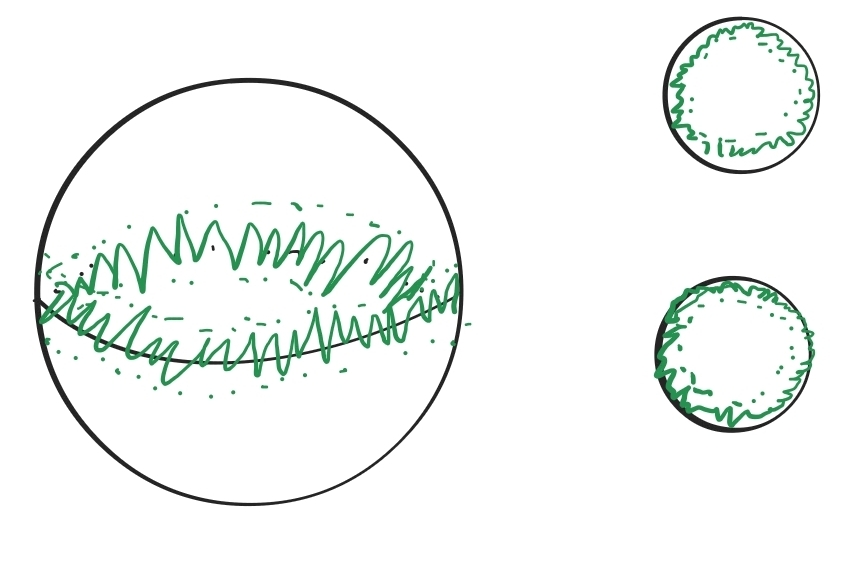
\includegraphics[width=0.5\textwidth]{projection-continuity}

	Bijectivity allows us to think about $\pi^{-1}$, which is also continuous by similar arguments.
	It appears that $\pi \circ \pi^{-1} = \id_{S_2\vee S^2}$ and $\pi^{-1} \circ \pi = \id_{S^2 / S^1}$, so this is not only a homotopy equivalence but in fact a homeomorphism.
\end{proof}

\begin{ex}
	The \textit{equator} of $S^3$ is the 2-sphere \begin{equation*}
		S^2 = \left\lbrace (x, y, z, 0) \in \mathbb{R}^4 : x^2 + y^2 + z^2 = 1 \right\rbrace.
	\end{equation*}
	Show that the inclusion map $j : S^2 \hookrightarrow S^3$ is homotopic to the constant map.
\end{ex}
\begin{proof}
	We will think of $S^3$ as $\mathbb{R}^3$ with a point $\infty$ at infinity so that we can use spherical coordinates to rewrite $S^2$ with the simple formula \begin{equation*}
		S^2 = \left\lbrace (1, \theta, \phi) \right\rbrace.
	\end{equation*}
	Note that we are using spherical coordinates for both $S^3$ realized as $\mathbb{R}^3$ with a point at infinity as well as the standard $\mathbb{R}^3$ that $S^2$ is sitting in, though in the former case we also include the point $\infty$.
	Thus the inclusion $i$ maps $(r, \theta, \phi) \mapsto (r, \theta, \phi)$, and the map $F : S^2 \times [0, 1] \to \mathbb{R}^3$ defined by $F((1, \theta, \phi), t) = (1-t, \theta, \phi)$ is a homotopy from $i$ to the constant map $c : (r, \theta, \phi) \mapsto (0, 0, 0)$ (note that $(0, \theta, \phi) = (0, 0, 0)$ for any choice of $\theta$ and $\phi$).
\end{proof}

\begin{ex}
	Let $T^2 = S^1 \times S^1$ be the 2-torus and $p \in T^2$ be any point.
	Show that $T^2 \setminus \lbrace p \rbrace$ deformation retracts to $S^1 \vee S^1$, the wedge product of two circles.
	A sequence of pictures exhibiting the deformation is perfectly fine.
\end{ex}
\begin{proof}
	Here, we have realized $T^2$ minus a point as its fundamental polygon minus a point.
	\\
	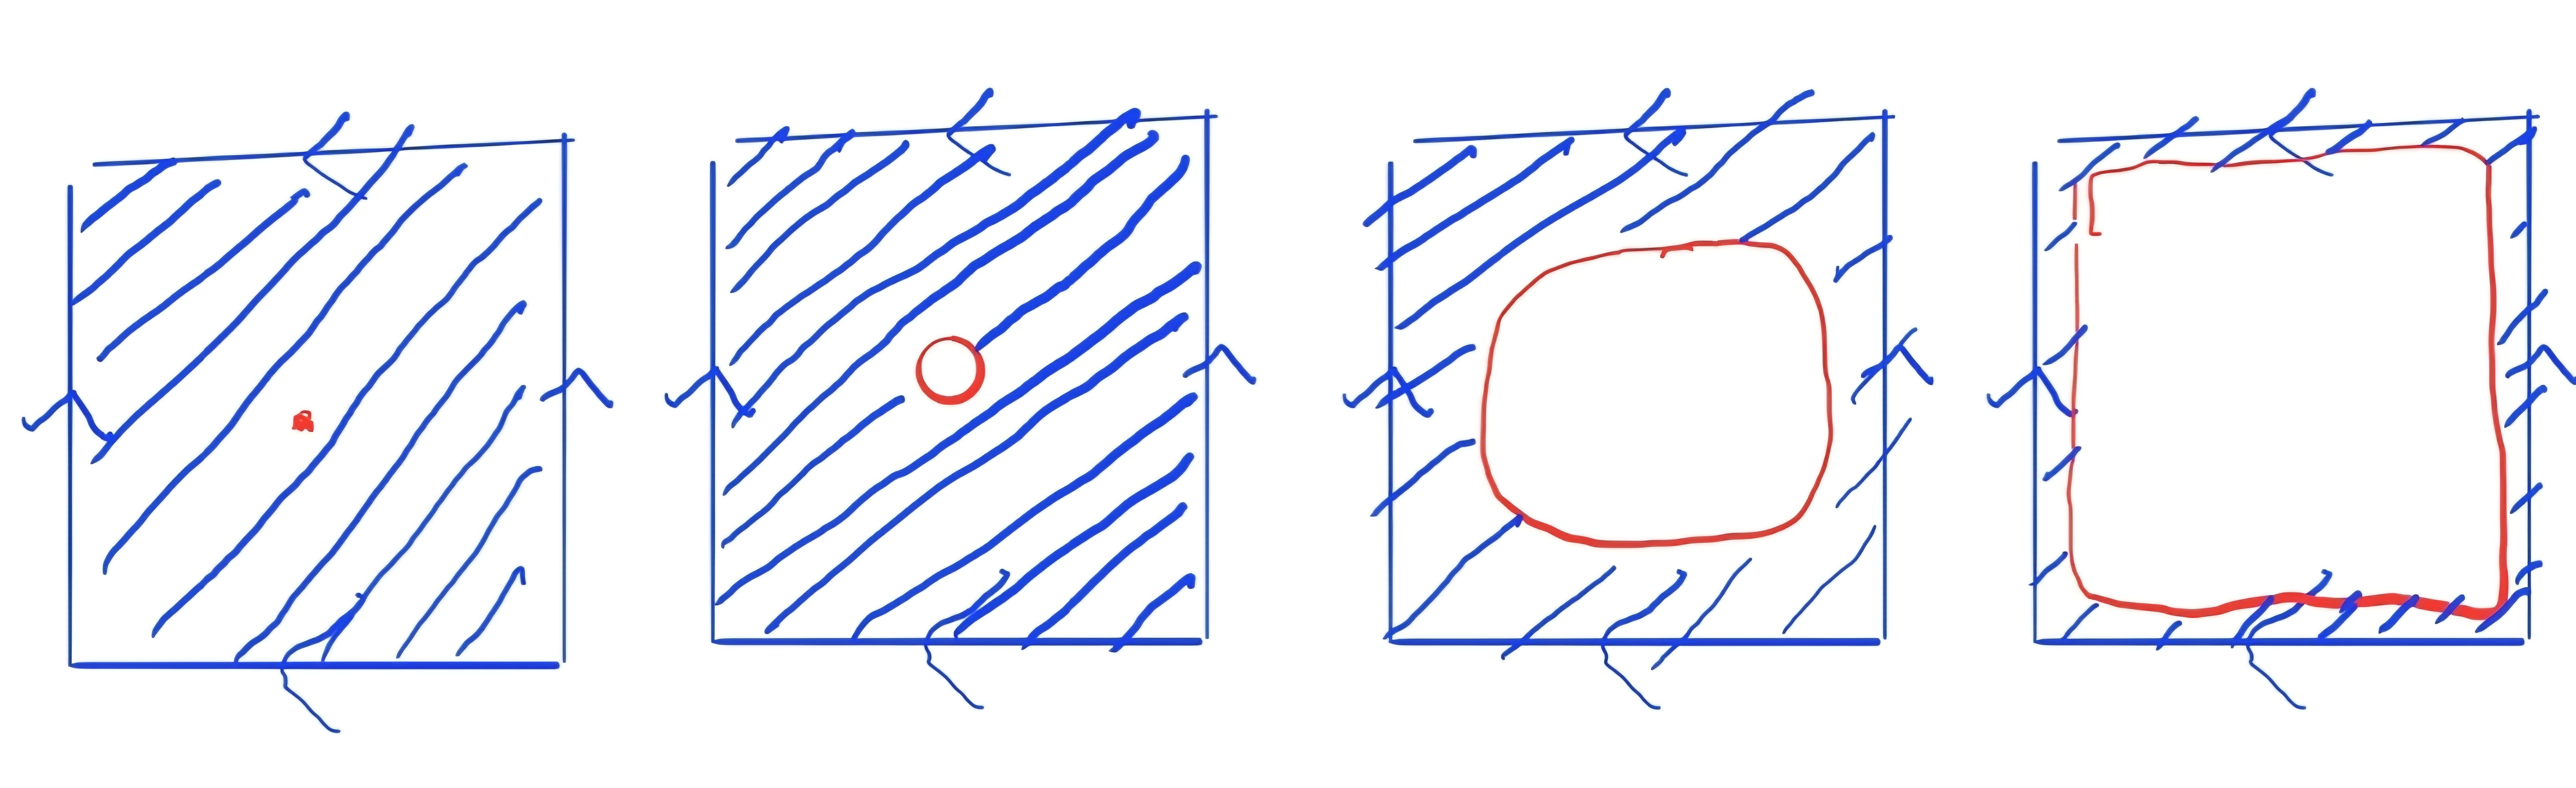
\includegraphics[width=0.5\textwidth]{pointless-torus}
	\\
	After the pictured final step, we should imagine the red taking up all the space except the boundary of the square.
	Then we have deformed the pointless torus to the boundary of the square, which is itself $S^1 \vee S^1$ (where the top and bottom together form one $S^1$, the left and right form the other, and the join point is the four corners).
\end{proof}

\begin{ex}
	Show that a contractible space is path-connected.
\end{ex}
\begin{proof}
	If a space $X$ is contractible, then there are maps $\varphi : X \to *$ and $\psi : * \to X$ such that $\psi \circ \varphi \simeq \id_X$ and $\varphi \circ \psi = \id_{*}$, where equality is achieved in the latter case because $\id_{*}$ is the only map from $* \to *$.
	Let $f = \psi \circ \varphi$ and let $p$ be the single point in the image of $f$.
	Let $F : X \times [0, 1] \to X$ be a homotopy from $\id_X$ to $f$.
	Then given two points $x, y \in X$, the path $(t \mapsto F_t(x)) * (t \mapsto F_{1-t}(y))$ takes $x$ to $y$ by passing through $p$, so $X$ is path-connected.
\end{proof}

\begin{ex}
	Find a circle $C \subset T^2$ and an explicit retraction $r : T^2 \to C$.
	Whether or not a retraction exists depends on the circle you pick.
\end{ex}
\begin{proof}
	We realize $T^2$ as its fundamental polygon $[0, 1] \times [0, 1]$ (first picture).
	Define \begin{equation*}
		C = \lbrace (0.75, y) : y \in [0, 1] \rbrace.
	\end{equation*}
  Then the map $r : (x, y) \mapsto (0.75, y)$ (first picture below) satisfies $r(T^2) \subset C$, it restricts to the identity on $C$, and it is continuous by the second and third pictures below, where the red line is $C$ and the blue areas indicate open sets.
  Thus $r$ is a retraction.
  \\
	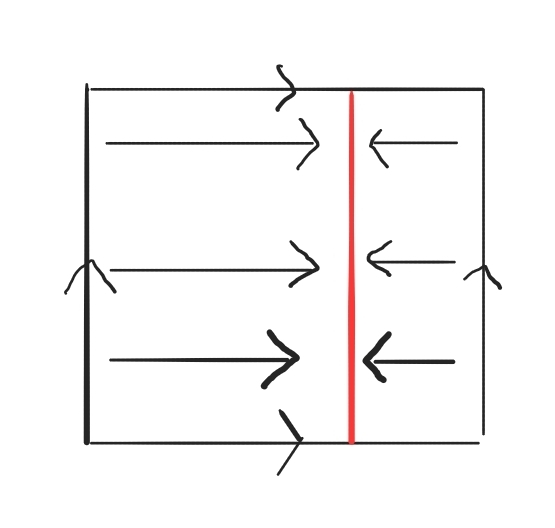
\includegraphics[width=0.3\textwidth]{retraction}
	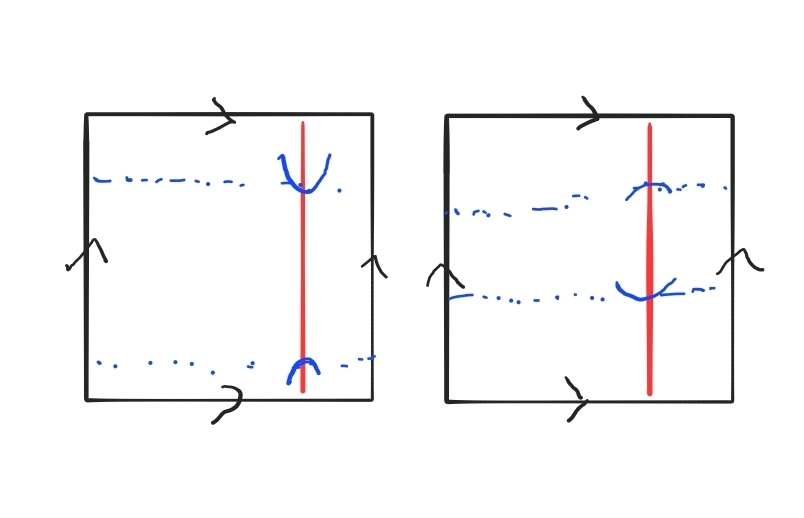
\includegraphics[width=0.45\textwidth]{retraction-continuity}
\end{proof}

\end{document}
